\lab{Latent Dirichlet Allocation}{Latent Dirichlet Allocation}
\objective{Understand the how to do topic analysis with LDA via a collapsed Gibbs sampler.}

Latent Dirichlet Allocation (LDA) is a generative model explaining how text documents are created. It supposes that there is some fixed vocabulary of terms (of length $V$) and $K$ different topics, each represented as a probability distribution $\phi_{k}$ over the vocabulary, each with a Dirichlet prior $\beta$. It further assumes that when a new document is to be generated, a probability distribution $\theta_{m}$ over the topics is drawn from a Dirichlet distribution with parameter $\alpha$. Then for each word in the document, we draw a topic assignment $z_{m,n}$ from the categorical distribution $\theta_{m}$, and then we draw a term assignment from the categorical distribution $\phi_{z_{m,n}}$. Throughout this implementation, we assume $\alpha$ and $\beta$ are scalars. In summary, we have
\begin{enumerate}
	\item Draw $\phi_{k} \sim \text{Dir}(\beta)$ for $1 \leq k \leq K$.
	\item Draw $\theta_{m} \sim \text{Dir}(\alpha)$ for $1 \leq m \leq D$.
	\begin{enumerate}
		\item Draw $z_{m,n} \sim \text{Cat}(\theta_{m})$ for $1 \leq n \leq N_{m}$.
		\item Draw $w_{m,n} \sim \text{Cat}(\phi_{z_{m,n}}$ for $1 \leq n \leq N_{m}$.
	\end{enumerate}
\end{enumerate}
This is typically depicted with graphical plate notation as in Figure \ref{fig:ldaplates}.
\begin{figure}[h]
\centering
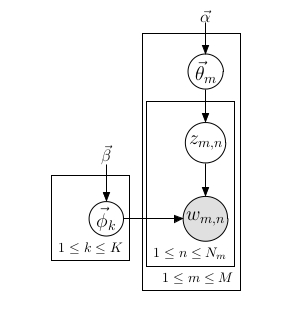
\includegraphics[width=\textwidth]{graphicalplate.jpg}
\caption{Graphical plate notation for LDA text generation.}
\label{fig:ldaplates}
\end{figure}

In the plate model, only the variables $w_{m,n}$ are shaded, signifying that these are the only observations visible to us; the rest are latent variables. We would like to be able to do two things: estimate each $\phi_{k}$ and each $\theta_{m}$. This will allow us to understand what each topic is, as well as understand how each document is distributed over the $K$ topics. We can estimate these well if we know $z_{m,n}$ for each $m, n$, collectively referred to as $\mathbf{z}$. It is intractable to sample directly from the joint posterior distribution $\mathbb{P}(\mathbf{z} | \mathbf{w}, \alpha, \beta)$ where $\mathbf{w}$ is the collection of term assignments in the text corpus. However, letting $\mathbf{z}_{\neg (m,n)} = \mathbf{z} - z_{m,n}$, the conditional posterior distributions $$\mathbb{P}(z_{m,n} = k | \mathbf{z}_{\neg (m,n)}, \mathbf{w}, \alpha, \beta)$$ have nice, closed form solutions, making them easy to sample from.

These conditional distributions have the following form:
\begin{equation*}
\mathbb{P}(z_{m,n} = k | \mathbf{z}_{\neg (m,n)}, \mathbf{w}, \alpha, \beta) \propto \frac{(n_{(k,m,\cdot)}^{\neg (m,n)} + \alpha)\cdot(n_{(k, \cdot, w_{m,n})}^{\neg (m,n)} + \beta)}{n_{(k,\cdot,\cdot)}^{\neg (m,n)} + V \cdot \beta}
\end{equation*}
where 
\begin{align*}
n_{(k,m,\cdot)} & = \mbox{ the number of words in document $m$ assigned to topic $k$} \\
n_{(k,\cdot,v)} & = \mbox{ the number of times term $v = w_{m,n}$ is assigned to topic $k$} \\
n_{(k,\cdot,\cdot)} & = \mbox{ the number of times topic $k$ is assigned in the corpus} \\
n_{(k,m,\cdot)}^{\neg (m,n)} & = n_{(k,m,\cdot)} - \indicator{z_{m,n} = k} \\
n_{(k,\cdot,v)}^{\neg (m,n)} & = n_{(k,\cdot,v)} - \indicator{z_{m,n} = k} \\
n_{(k,\cdot,\cdot)}^{\neg (m,n)} & = n_{(k,\cdot,\cdot)} - \indicator{z_{m,n} = k}
\end{align*}

Thus, if we simply keep track of these count matrices, then we can easily create a Gibbs sampler over the topic assignments. This is actually a particular class of samplers known as \emph{collapsed Gibbs samplers}, because we have collapsed the sampler by integrating out $\theta$ and $\phi$.

We have provided for you the structure of a Python object \li{LDACGS} with several methods. The object is already defined to have attributes \li{n\_topics, documents, vocab, alpha} and \li{beta}, where \li{vocab} is a list of strings (terms), and documents is a list of dictionaries (a dictionary for each document). Each entry in dictionary $m$ is of the form $n : w$, where $w$ is the index in \li{vocab} of the $n^{th}$ word in document $m$.

Throughout this lab we will guide you through writing several more methods in order to implement the Gibbs sampler. The first step is to initialize our assignments, and create the count matrices $n_{(k,m,\cdot)}, n_{(k,\cdot,v)}$ and vector $n_{(k,\cdot,\cdot)}$.

\begin{problem}
Complete the method \li{initialize}. By randomly assigning initial topics, fill in the count matrices and topic assignment dictionary.
\end{problem}

The next method we need to write fully outlines a sweep of the Gibbs sampler.

\begin{problem}
Complete the method \li{\_sweep}, which needs to iterate through each word of each document. It should call on the method \li{\_conditional} to get the conditional distribution at each iteration.
\end{problem}

We need to write the method to create the appropriate conditional distribution.

\begin{problem}
Complete the method \li{\_conditional}. It accepts arguments $m,w$ where $m$ is the document and $w$ is an index of \li{vocab}. Don't forget to normalize to ensure you are actually returning a distribution!
\end{problem}

We are now prepared to write the full Gibbs sampler.

\begin{problem}
Complete the method \li{sample}. The argument \emph{filename} is the name and location of a .txt file, where each line is considered a document. The corpus is built by method \li{buildCorpus}, and stopwords are removed (if argument \emph{stopwords} is provided). Burn in the Gibbs sampler, computing and saving the log-likelihood with the method \li{\_loglikelihood}. After the burn in, iterate further, accumulating your count matrices, by adding \li{nzw} and \li{nmz} to \li{total\_nzw} and \li{total\_nmz} respectively, where you only add every \emph{sample\_rate}$^{th}$ iteration. Also save each log-likelihood.
\end{problem}

You should now have a working Gibbs sampler to perform LDA inference on a corpus. Let's test it out on Ronald Reagan's State of the Union addresses.

\begin{problem}
Create an \li{LDACGS} object with $20$ topics, letting \li{alpha} and \li{beta} be the default values. Load in the stop word list provided. Run the Gibbs sampler, with a burn in of $100$ iterations, accumulating $10$ samples, only keeping the results of every $10$ sweep. Plot the log-likelihoods. How long did it take to truly burn in?
\end{problem}

We can estimate the values of each $\phi_{k}$ and each $\theta_{m}$ as follows:

\begin{align*}
\widehat{\theta}_{m,k} & = \frac{n_{(k,m,\cdot)} + \alpha}{K \cdot \alpha + \sum_{k=1}^{K} n_{(k,m,\cdot)}} \\
\widehat{\phi}_{k,v} & = \frac{n_{(k,\cdot,v)} + \beta}{V \cdot \beta + \sum_{v=1}^{V} n_{(k,\cdot,v)}}
\end{align*}

We have provided methods \li{phi} and \li{theta} that do this for you. We often examine the topic-term distributions $\phi_{k}$ by looking at the $n$ terms with highest probability, where $n$ is small (say $10$ or $20$).  We have provided a method \li{topterms} which does this for you.

\begin{problem}
Using the methods described above, examine the topics for Reagan's addresses. As best as you can, come up with labels for each topic.
\end{problem}

We can use $\widehat{\theta}$ to find the paragraphs in Reagan's addresses that focus the most on each topic. The documents with highest values of $\widehat{\theta}_{k}$ are those most heavily focused on topic $k$.

\begin{problem}
In your above topic analysis, you should have found a topic about the Cold War and one about education. Find the five paragraphs in Reagan's addresses that most closely focus on each of these topics, according to the above method.
\end{problem}